\documentclass[11pt, letterpaper]{article}

% ----- Packages -----
\usepackage{amsmath, amssymb, amsthm}
\usepackage{geometry}
\usepackage{tikz}
\usetikzlibrary{arrows.meta, positioning, shapes.geometric, calc}
\usepackage{mathrsfs}
\usepackage{mathtools}
\usepackage{enumitem}
\usepackage{xcolor}
\usepackage{hyperref}

% ----- Page Setup -----
\geometry{top=1in, bottom=1in, left=1in, right=1in}
\setlength{\parindent}{0pt}
\setlength{\parskip}{0.5em}

% ----- Theorem Environments -----
\newtheorem{theorem}{Theorem}[section]
\newtheorem{lemma}[theorem]{Lemma}
\newtheorem{corollary}[theorem]{Corollary}
\newtheorem{proposition}[theorem]{Proposition}
\theoremstyle{definition}
\newtheorem{definition}[theorem]{Definition}
\newtheorem{example}[theorem]{Example}
\newtheorem{problem}{Problem}[section]
\theoremstyle{remark}
\newtheorem{remark}[theorem]{Remark}

% ----- Custom Commands -----
\newcommand{\Z}{\mathbb{Z}}
\newcommand{\R}{\mathbb{R}}
\newcommand{\N}{\mathbb{N}}
\newcommand{\Q}{\mathbb{Q}}
\newcommand{\E}{\mathbb{E}}
\newcommand{\F}{\mathcal{F}}
\renewcommand{\P}{\mathbb{P}}

\title{\textbf{Homework 3.5 \& Chapter Review: Mathematical Proof Techniques}\\ \Large Direct, Contrapositive, and Proof by Cases}
\author{Tashfeen Omran}
\date{September 2026}

\begin{document}

\maketitle
\tableofcontents
\newpage

% ==========================================
% PART 1: INTRODUCTION
% ==========================================
\section{Part 1: Comprehensive Introduction, Context, and Prerequisites}

\subsection{Core Concepts, Axioms, and Intuition}
Abstract mathematics requires more than computational arithmetic; it requires absolute logical certainty derived from foundational axioms. The transition from computational calculus to abstract mathematics hinges on the concept of the \textbf{formal proof}: a finite sequence of logical deductions starting from accepted axioms and arriving at a necessarily true conclusion.

In this chapter, we explore three primary architectures of logical deduction:
\begin{enumerate}
    \item \textbf{Direct Proof:} To prove an implication $P \implies Q$, we assume $P$ is true and use axioms, definitions, and previously established theorems to deduce that $Q$ must also be true.
    \item \textbf{Proof by Contrapositive:} In propositional logic, an implication $P \implies Q$ is logically equivalent to its contrapositive $\neg Q \implies \neg P$. If the negation of the conclusion provides a more algebraically tractable starting point, we assume $\neg Q$ and derive $\neg P$.
    \item \textbf{Proof by Cases (Exhaustion):} If the domain of our hypothesis can be partitioned into a set of mutually exclusive and collectively exhaustive subsets (e.g., all integers are either even or odd), we can prove the theorem by showing it holds within every individual subset. 
\end{enumerate}

\textbf{Intuition via Set Theory:} Think of $P$ and $Q$ as defining sets of objects, $A$ and $B$, for which the statements are true. The implication $P \implies Q$ is equivalent to asserting that $A \subseteq B$. A direct proof takes an arbitrary $x \in A$ and shows $x \in B$. A contrapositive proof takes an arbitrary $x \notin B$ (outside the larger set) and shows $x \notin A$ (it cannot be in the smaller set). 

\subsection{Historical Context and Motivation}
The formalization of logical proof dates back to Aristotle's syllogistic logic and Euclid's \textit{Elements}, which established the axiomatic method geometry. However, the foundational crisis of mathematics in the late 19th and early 20th centuries (spurred by paradoxes discovered by Bertrand Russell and formalized by Gottlob Frege) required mathematicians to rigorously define what constitutes a valid proof. Today's proof techniques form the bedrock of Zermelo-Fraenkel set theory (ZFC), the standard foundation for modern mathematics and formal verification in computer science.

\subsection{Key Theorems, Lemmas, and Equivalences}
\begin{itemize}
    \item \textbf{Law of the Excluded Middle:} For any proposition $P$, $P \lor \neg P$ is true. (Fundamental for proof by cases).
    \item \textbf{Logical Equivalence of Contrapositive:} $(P \implies Q) \iff (\neg Q \implies \neg P)$.
    \item \textbf{De Morgan's Laws:} $\neg(P \lor Q) \iff (\neg P \land \neg Q)$ and $\neg(P \land Q) \iff (\neg P \lor \neg Q)$.
    \item \textbf{Parity Definitions:} An integer $n \in \Z$ is even if $\exists k \in \Z$ such that $n = 2k$. It is odd if $\exists k \in \Z$ such that $n = 2k + 1$. 
\end{itemize}

\subsection{Prerequisites}
To fully master these topics, one must be comfortable with:
\begin{itemize}
    \item \textbf{Basic Set Theory:} Understanding unions $\cup$, intersections $\cap$, set differences, and subsets.
    \item \textbf{Algebraic Manipulation of Integers:} Expanding polynomials, factoring, and recognizing multiples.
    \item \textbf{Propositional Logic:} Truth tables, negation of compound statements, and biconditionals ($P \iff Q$).
\end{itemize}

\newpage

% ==========================================
% PART 2: DETAILED HOMEWORK SOLUTIONS
% ==========================================
\section{Part 2: Detailed Homework Solutions (Rigorous Proofs)}

\subsection{Section 3.5 Exercises: Proof Evaluations}

\textbf{Problem 3.41} \\
\textit{Evaluate the given proof.}
\begin{proof}[Solution Analysis]
The provided proof partitions the domain into two cases: Case 1 assumes $a$ and $b$ are even; Case 2 assumes $a$ and $b$ are odd. In both cases, it successfully derives that $a^2 - b^2$ is even. 
The assumption "Case 1: $a$ and $b$ are even, Case 2: $a$ and $b$ are odd" is logically equivalent to assuming "$a$ and $b$ are of the same parity."
Therefore, the result that is actually being proved is: \textbf{(3) Let $a, b \in \Z$. If $a$ and $b$ are of the same parity, then $a^2 - b^2$ is even.}
\end{proof}

\textbf{Problem 3.42} \\
\textit{Below is given a proof of a result. Which result is being proved?}
\begin{proof}[Solution Analysis]
The proof consists of two parts. The first part begins by assuming $x$ is even ($x=2a$) and deduces that $3x^2 - 4x - 5 = 2(6a^2 - 4a - 3) + 1$, which is odd. 
The second part is explicitly labeled "For the converse," assumes $x$ is odd ($x=2b+1$), and deduces that $3x^2 - 4x - 5 = 2(6b^2 + 2b - 3)$, which is even. 
By proving $P \implies Q$ (where $P$ is "$x$ is even" and $Q$ is "$3x^2 - 4x - 5$ is odd") and $\neg P \implies \neg Q$ (which is the contrapositive of $Q \implies P$), the author has proven the biconditional.
Result proved: \textbf{Let $x \in \Z$. Then $x$ is even if and only if $3x^2 - 4x - 5$ is odd.}
\end{proof}

\textbf{Problem 3.43} \\
\textit{Evaluate the proof of the following result: Let $n \in \Z$. If $3n-8$ is odd, then $n$ is odd.}
\begin{proof}[Solution Analysis]
The stated theorem is of the form $P \implies Q$. The proof begins with "Assume that $n$ is odd." It then derives that $3n-8$ is odd. This is a proof of $Q \implies P$, which is the \textbf{converse} of the theorem. Proving the converse does not prove the original implication. Therefore, the proof is mathematically invalid for the stated result.
\end{proof}

\textbf{Problem 3.44} \\
\textit{Evaluate the proof of the result: Let $a,b \in \Z$. Then $a-b$ is even if and only if $a$ and $b$ are of the same parity.}
\begin{proof}[Solution Analysis]
The result is a biconditional statement ($P \iff Q$). The proof only uses two cases: both even, and both odd. This correctly proves the "if" direction: $a,b$ same parity $\implies a-b$ is even. However, the proof \textbf{completely omits the converse} (or the other cases: one even, one odd). Furthermore, within Subcase 1.1, the variables $x$ and $y$ are poorly managed; writing $a=2x$ and $b=2y$ is fine, but re-using $x,y$ in Subcase 1.2 ($a=2x+1, b=2y+1$) is formally acceptable but poor style. The main logical error is the omission of the converse proof.
\end{proof}

\textbf{Problem 3.45} \\
\textit{The following is an attempted proof of a result. What is the result and is the attempted proof correct?}
\begin{proof}[Solution Analysis]
The proof states "Assume, without loss of generality, that $x$ is even. Then $x=2a$..." and concludes $xy^2$ is even. 
Result proven: \textbf{If $x$ is an even integer, then $xy^2$ is an even integer for any integer $y$.}
Is the proof correct? The phrase "without loss of generality" (WLOG) implies that the original result was symmetric with respect to $x$ and $y$ (e.g., "If $x$ or $y$ is even, then $xy^2$ is even"). If that was the result, WLOG is invalid because $x$ and $y$ do not have symmetric roles in the expression $xy^2$. Thus, either the WLOG is erroneously included, or the proof fails to check the case where $y$ is even and $x$ is odd.
\end{proof}

\textbf{Problem 3.46} \\
\textit{Given below is a proof of a result. What is the result?}
\begin{proof}[Solution Analysis]
The proof begins with "Assume, without loss of generality, that $x$ and $y$ are even. Then $x=2a$ and $y=2b$..." It concludes that $xy + xz + yz$ is even.
Result proved: \textbf{Let $x, y, z \in \Z$. If $x$ and $y$ are even, then $xy+xz+yz$ is even.} 
The use of WLOG here indicates the author might have been proving "If any two of $x,y,z$ are even, then $xy+xz+yz$ is even." Since the expression is perfectly symmetric with respect to permutations of $x,y,z$, the WLOG is mathematically justified.
\end{proof}

\textbf{Problem 3.47} \\
\textit{What result is being proved below and what procedure is being used?}
\begin{proof}[Solution Analysis]
The proof is split into two phases. 
Phase 1 (Lemma): "Assume $x$ is even... Thus $7x-3$ is odd." This proves $x \text{ even} \implies 7x-3 \text{ odd}$. By contrapositive, $7x-3 \text{ even} \implies x \text{ odd}$.
Phase 2 (Main): "Assume $7x-3$ is even. From the result above, $x$ is odd... Thus $3x+8$ is odd."
Result proved: \textbf{Let $x \in \Z$. If $7x-3$ is even, then $3x+8$ is odd.} 
Procedure: Direct proof utilizing a previously proven lemma (or establishing a sub-result first to determine the parity of $x$).
\end{proof}

\textbf{Problem 3.48} \\
\textit{Which would be an appropriate way to begin a proof of: $(n-5)(n+7)(n+13)$ is odd if and only if $n$ is even?}
\begin{proof}[Solution Analysis]
Since this is a biconditional statement regarding the parity of an expression entirely dependent on $n$, the most comprehensive and standard approach is to partition the integers into parity classes. 
Appropriate choice: \textbf{(e) We consider two cases, according to whether $n$ is even or $n$ is odd.} This will naturally prove both directions of the biconditional simultaneously.
\end{proof}

\subsection{Chapter 3 Supplemental Exercises}

\textbf{Problem 3.49:} Let $x \in \Z$. Prove that if $7x-8$ is even, then $x$ is even.
\begin{proof}
We proceed by contrapositive. Assume $x$ is odd. Then $x = 2k + 1$ for some integer $k$. We evaluate $7x - 8$:
\begin{align*}
    7x - 8 &= 7(2k + 1) - 8 \\
           &= 14k + 7 - 8 = 14k - 1 \\
           &= 2(7k - 1) + 1.
\end{align*}
Since $7k - 1 \in \Z$, $7x - 8$ is odd. By proving the contrapositive, the original statement is true.
\end{proof}

\textbf{Problem 3.50:} Let $x \in \Z$. Prove that $x^3$ is even if and only if $x$ is even.
\begin{proof}
($\impliedby$): Assume $x$ is even. Then $x = 2k$ for $k \in \Z$. $x^3 = (2k)^3 = 8k^3 = 2(4k^3)$. Since $4k^3 \in \Z$, $x^3$ is even. \\
($\implies$): We use the contrapositive. Assume $x$ is odd. Then $x = 2k+1$ for $k \in \Z$. 
\begin{align*}
    x^3 &= (2k+1)^3 = 8k^3 + 12k^2 + 6k + 1 \\
        &= 2(4k^3 + 6k^2 + 3k) + 1.
\end{align*}
Since $4k^3 + 6k^2 + 3k \in \Z$, $x^3$ is odd. Both directions hold.
\end{proof}

\textbf{Problem 3.51:} Let $x \in \Z$. Use lemmas to prove $3x^3$ is even if and only if $5x^2$ is even.
\begin{proof}
Lemma 1: $x$ is even $\iff$ $3x^3$ is even. (Proof: If $x=2k$, $3x^3 = 24k^3 = 2(12k^3)$ even. If $x=2k+1$, $3x^3 = 3(8k^3+12k^2+6k+1) = 2(12k^3+18k^2+9k+1)+1$ odd). \\
Lemma 2: $x$ is even $\iff$ $5x^2$ is even. (Proof: If $x=2k$, $5x^2 = 20k^2 = 2(10k^2)$ even. If $x=2k+1$, $5x^2 = 5(4k^2+4k+1) = 2(10k^2+10k+2)+1$ odd). \\
By transitivity of the biconditional operator: ($3x^3$ is even) $\iff$ ($x$ is even) $\iff$ ($5x^2$ is even).
\end{proof}

\textbf{Problem 3.52:} Give a direct proof of: Let $x \in \Z$. If $11x-5$ is odd, then $x$ is even.
\begin{proof}
Assume $11x-5$ is odd. Then $11x-5 = 2k+1$ for some $k \in \Z$. 
Notice that $11x = 2k+6$. We can rewrite $11x$ as $x + 10x$. 
So, $x + 10x = 2k + 6 \implies x = 2k + 6 - 10x = 2(k + 3 - 5x)$.
Since $x$ and $k$ are integers, $k+3-5x \in \Z$. Thus, $x$ is an even integer.
\end{proof}

\textbf{Problem 3.53:} Let $x, y \in \Z$. Prove that if $x+y$ is odd, then $x$ and $y$ are of opposite parity.
\begin{proof}
We proceed by contrapositive. Assume $x$ and $y$ are of the same parity. 
Case 1 ($x, y$ both even): $x=2a, y=2b \implies x+y = 2a+2b = 2(a+b)$, which is even.
Case 2 ($x, y$ both odd): $x=2a+1, y=2b+1 \implies x+y = 2a+2b+2 = 2(a+b+1)$, which is even.
In all cases, $x+y$ is even (not odd). The contrapositive is proven.
\end{proof}

\textbf{Problem 3.54:} Let $x, y \in \Z$. Prove that if $3x+5y$ is even, then $x$ and $y$ are of the same parity.
\begin{proof}
We proceed by contrapositive. Assume $x$ and $y$ are of opposite parity.
Case 1 ($x$ even, $y$ odd): $x=2a, y=2b+1$. Then $3x+5y = 3(2a) + 5(2b+1) = 6a + 10b + 5 = 2(3a+5b+2) + 1$, which is odd.
Case 2 ($x$ odd, $y$ even): $x=2a+1, y=2b$. Then $3x+5y = 3(2a+1) + 5(2b) = 6a + 3 + 10b = 2(3a+5b+1) + 1$, which is odd.
In both cases, $3x+5y$ is odd. The contrapositive is proven.
\end{proof}

\textbf{Problem 3.55:} Let $x, y \in \Z$. Prove that $(x+1)^2$ is even if and only if $x$ is odd or $y$ is even.
\begin{proof}
\textit{Note:} The statement as written in the textbook is logically flawed due to the inclusion of $y$. We will demonstrate this via counterexample, then prove the corrected statement.
If $x=2$ and $y=2$. The premise "$(x+1)^2$ is even" evaluates to $3^2=9$ is even (False). The conclusion "$x$ is odd or $y$ is even" evaluates to "False or True" (True). Thus, False $\iff$ True, which is a contradiction.
\textbf{Corrected result to prove:} $(x+1)^2$ is even $\iff x$ is odd.
($\impliedby$): Assume $x$ is odd. Then $x=2k+1$. $(x+1)^2 = (2k+2)^2 = 4(k+1)^2 = 2(2(k+1)^2)$, which is even.
($\implies$): Assume $x$ is even (contrapositive). $x=2k$. $(x+1)^2 = (2k+1)^2 = 4k^2+4k+1 = 2(2k^2+2k)+1$, which is odd.
\end{proof}

\textbf{Problem 3.56:} Let $x,y \in \Z$. Prove that if $xy$ and $x+y$ are even, then both $x$ and $y$ are even.
\begin{proof}
We use contrapositive: if it is not the case that both $x$ and $y$ are even, then either $xy$ is odd or $x+y$ is odd.
Assume it is not the case that both are even. 
Case 1: Both $x$ and $y$ are odd. $x=2a+1, y=2b+1$. Then $xy = (2a+1)(2b+1) = 4ab+2a+2b+1 = 2(2ab+a+b)+1$, which is odd. Thus, it's false that $xy$ and $x+y$ are even.
Case 2: One is even, one is odd. WLOG, $x=2a, y=2b+1$. Then $x+y = 2a+2b+1 = 2(a+b)+1$, which is odd. Thus, it's false that $xy$ and $x+y$ are even.
In all cases, the contrapositive holds.
\end{proof}

\textbf{Problem 3.57:} Prove that for every integer $x$, the integers $3x+1$ and $5x+2$ are of opposite parity.
\begin{proof}
Consider the sum of the two integers:
$(3x+1) + (5x+2) = 8x + 3 = 8x + 2 + 1 = 2(4x+1) + 1$.
Since $4x+1 \in \Z$, the sum is an odd integer. It is a fundamental lemma that if the sum of two integers is odd, they must be of opposite parity (proven in 3.53). Thus, $3x+1$ and $5x+2$ are of opposite parity.
\end{proof}

\textbf{Problem 3.58:} Prove (a) If $n^3$ is even, $n$ is even. (b) If $n$ is an odd integer, then $5n^9 + 13$ is even.
\begin{proof}
(a) Contrapositive: Assume $n$ is odd. $n=2k+1$. $n^3 = 8k^3+12k^2+6k+1 = 2(4k^3+6k^2+3k)+1$, which is odd.
(b) Direct: Assume $n$ is odd. By part (a) generalized, the product of odd integers is odd, so $n^9$ is odd. Let $n^9 = 2m+1$. Then $5n^9 + 13 = 5(2m+1) + 13 = 10m + 18 = 2(5m + 9)$. Since $5m+9 \in \Z$, $5n^9+13$ is even.
\end{proof}

\textbf{Problem 3.59:} Prove for every two distinct real numbers $a,b$ that either $\frac{a+b}{2} > a$ or $\frac{a+b}{2} > b$.
\begin{proof}
We proceed by contradiction. Assume there exist distinct real numbers $a,b$ such that $\frac{a+b}{2} \le a$ and $\frac{a+b}{2} \le b$.
Adding the two inequalities yields:
$\frac{a+b}{2} + \frac{a+b}{2} \le a + b \implies a+b \le a+b$.
While this is not a strict contradiction itself, let's solve the individual inequalities:
$\frac{a+b}{2} \le a \implies a+b \le 2a \implies b \le a$.
$\frac{a+b}{2} \le b \implies a+b \le 2b \implies a \le b$.
Thus, $a \le b$ and $b \le a$, which forces $a=b$. But the hypothesis states $a$ and $b$ are distinct ($a \neq b$). Contradiction.
\end{proof}

\textbf{Problem 3.60:} Let $x, y \in \Z$. Prove that if $a$ and $b$ are even integers, then $ax+by$ is even.
\begin{proof}
Assume $a$ and $b$ are even. Then $a = 2k$ and $b = 2m$ for integers $k,m$.
Then $ax+by = (2k)x + (2m)y = 2(kx + my)$.
Since $k,x,m,y \in \Z$, $kx+my \in \Z$. Thus $ax+by$ is even.
\end{proof}

\textbf{Problem 3.61:} Evaluate the proof...
\begin{proof}[Solution Analysis]
The theorem states: Let $x, y \in \Z$ and $a,b$ be odd. If $ax+by$ is even, then $x$ and $y$ are of the same parity.
The proof starts by assuming $x$ and $y$ are of opposite parity. It then sets $x=2p, y=2q+1$ and uses the fact that $a=2r+1, b=2s+1$. It calculates $ax+by$ and perfectly demonstrates it factors to $2(\text{integer}) + 1$, making it odd.
The proof correctly applies the contrapositive technique and accurately manipulates the algebra. \textbf{Evaluation: The proof is completely mathematically correct and logically sound.}
\end{proof}

\textbf{Problem 3.62:} Let $S=\{a,b,c,d\}$ be 4 distinct integers. Prove if (1) each $x \in S$ and the sum of any two remaining are same parity, OR (2) opposite parity, then every pair is same parity.
\begin{proof}
Let $T$ be any subset of 3 elements from $S$. 
Case 1: For any $x \in S$, $x$ and the sum of 2 of the remaining 3 are the same parity. Let $x_1 \in S$, and let $x_2, x_3, x_4$ be the rest. We are given $x_1 \equiv x_2+x_3 \pmod 2$. By symmetry of the rule, $x_2 \equiv x_1+x_3 \pmod 2$. 
Subtracting these congruences: $x_1 - x_2 \equiv x_2 - x_1 \pmod 2 \implies 2x_1 - 2x_2 \equiv 0 \pmod 2$, which is trivially true. 
Let's add them: $x_1 + x_2 \equiv x_1 + x_2 + 2x_3 \equiv x_1 + x_2 \pmod 2$, also trivial.
Notice that we have $x_1 \equiv x_2+x_3 \pmod 2$ and $x_1 \equiv x_2+x_4 \pmod 2$. 
Subtracting these yields $0 \equiv x_3 - x_4 \pmod 2 \implies x_3 \equiv x_4 \pmod 2$. By applying this to all combinations, all elements are mutually congruent mod 2 (they have the same parity).
Case 2: For any $x \in S$, opposite parity. $x_1 \equiv x_2+x_3+1 \pmod 2$ and $x_1 \equiv x_2+x_4+1 \pmod 2$. Subtracting yields $0 \equiv x_3-x_4 \pmod 2 \implies x_3 \equiv x_4 \pmod 2$. Again, all elements have the same parity. 
\end{proof}

\textbf{Problem 3.63:} Prove that if $a, b \in \Z^+$, then $a^2(b+1) + b^2(a+1) \ge 4ab$.
\begin{proof}
Expand the left side:
$a^2b + a^2 + b^2a + b^2 = ab(a+b) + a^2 + b^2$.
Because $a,b$ are positive integers, $a \ge 1$ and $b \ge 1$. Hence, $a+b \ge 2$.
Therefore, $ab(a+b) \ge 2ab$. 
Furthermore, it is a well-known algebraic identity that $(a-b)^2 \ge 0 \implies a^2+b^2 \ge 2ab$.
Adding these two inequalities:
$ab(a+b) + a^2+b^2 \ge 2ab + 2ab = 4ab$.
\end{proof}

\textbf{Problem 3.64:} Let $a,b \in \Z$. Prove if $ab = 4$, then $(a-b)^3 - 9(a-b) = 0$.
\begin{proof}
Since $a,b \in \Z$ and $ab=4$, the possible pairs for $(a,b)$ are:
$(1,4), (4,1), (2,2), (-2,-2), (-1,-4), (-4,-1)$.
For each pair, let us calculate the difference $x = a-b$:
$1-4 = -3$, $4-1 = 3$, $2-2 = 0$, $-2-(-2)=0$, $-1-(-4)=3$, $-4-(-1)=-3$.
In all possible scenarios, $x = a-b \in \{-3, 0, 3\}$.
We want to show $x^3 - 9x = 0$. Factor the polynomial: $x^3 - 9x = x(x^2 - 9) = x(x-3)(x+3)$.
If $x=-3$, $(-3)(-6)(0) = 0$. If $x=0$, $0 = 0$. If $x=3$, $(3)(0)(6) = 0$.
In every case, $(a-b)^3 - 9(a-b) = 0$.
\end{proof}

\textbf{Problem 3.65:} $a \le b \le c$ sides of triangle $T$. Prove if $T$ is right, $(abc)^2 = (c^6 - a^6 - b^6)/3$.
\begin{proof}
Assume $T$ is a right triangle. Since $c$ is the longest side, by the Pythagorean theorem, $c^2 = a^2 + b^2$.
Cube both sides:
$(c^2)^3 = (a^2+b^2)^3 \implies c^6 = a^6 + 3a^4b^2 + 3a^2b^4 + b^6$.
$c^6 = a^6 + b^6 + 3a^2b^2(a^2+b^2)$.
Substitute $c^2$ back in for $(a^2+b^2)$:
$c^6 = a^6 + b^6 + 3a^2b^2c^2$.
Rearranging the terms:
$3(abc)^2 = c^6 - a^6 - b^6 \implies (abc)^2 = \frac{c^6 - a^6 - b^6}{3}$.
\end{proof}

\textbf{Problem 3.66:} Which is an appropriate way to begin proof of $3n^3+4n^2+5$ even $\iff n$ even?
\begin{proof}[Solution Analysis]
Since this is a biconditional involving powers of $n$ and parity, a direct approach proving both implications separately via cases on the parity of $n$ covers all integers comprehensively.
Appropriate choice: \textbf{(e) We consider two cases, according to whether $n$ is even or $n$ is odd.}
\end{proof}

\textbf{Problem 3.67:} Let $\mathcal{P} = \{A, B, C\}$ partition $S$. $A=\{n: n \text{ odd, } n>0\}$, $B=\{n: n \text{ odd, } n<0\}$, $C=\{n: n \text{ even, } n>0\}$. Prove if $x,y$ are in distinct subsets, $xy$ is odd, even and $>1$, or even and $<-1$.
\begin{proof}
By definition of the partition, $0 \notin A \cup B \cup C$ (since 0 is not odd, nor is it $>0$). So $x,y \neq 0$.
Case 1: $x \in A, y \in B$. $x$ is odd $>0$, $y$ is odd $<0$. The product of two odds is odd. $xy$ is odd.
Case 2: $x \in A, y \in C$ (or vice versa). $x$ is odd $>0$, $y$ is even $>0$. Product of even and odd is even. Since both are positive and non-zero, $x \ge 1$ and $y \ge 2$ (smallest positive even). Thus $xy \ge 2 > 1$. $xy$ is even and $>1$.
Case 3: $x \in B, y \in C$. $x$ is odd $<0$, $y$ is even $>0$. Product is even. $x \le -1, y \ge 2 \implies xy \le -2 < -1$. $xy$ is even and $<-1$.
Thus, the condition holds.
\end{proof}

\textbf{Problem 3.68:} Let $n \in \N$. Prove that if $n^3 - 5n - 10 > 0$, then $n \ge 3$.
\begin{proof}
We proceed by contrapositive. Assume $n \in \N$ but $n < 3$. 
Since $n$ is a natural number (positive integer), $n \in \{1, 2\}$.
If $n = 1$: $1^3 - 5(1) - 10 = -14 \le 0$.
If $n = 2$: $2^3 - 5(2) - 10 = 8 - 10 - 10 = -12 \le 0$.
In both cases, it is false that $n^3 - 5n - 10 > 0$. The contrapositive holds.
\end{proof}

\textbf{Problem 3.69:} Prove for every odd $a$ that $(a^2+3)(a^2+7) = 32b$ for some integer $b$.
\begin{proof}
Assume $a$ is odd. Then $a = 2k+1$.
$a^2 = 4k^2 + 4k + 1 = 4k(k+1) + 1$.
Since $k$ and $k+1$ are consecutive integers, their product $k(k+1)$ is even (let it be $2m$).
Thus, $a^2 = 4(2m) + 1 = 8m + 1$.
Substitute $a^2 = 8m+1$ into the expression:
$(8m+1+3)(8m+1+7) = (8m+4)(8m+8) = 4(2m+1) \cdot 8(m+1) = 32(2m+1)(m+1)$.
Let $b = (2m+1)(m+1)$. Since $m \in \Z$, $b \in \Z$, and the expression equals $32b$.
\end{proof}

\textbf{Problem 3.70:} Prove for every two positive integers $a, b$ that $(a+b)\left(\frac{1}{a} + \frac{1}{b}\right) \ge 4$.
\begin{proof}
Expand the product:
$(a+b)\left(\frac{1}{a} + \frac{1}{b}\right) = 1 + \frac{a}{b} + \frac{b}{a} + 1 = 2 + \frac{a}{b} + \frac{b}{a}$.
For any positive real numbers $x,y$, by AM-GM inequality, $x+y \ge 2\sqrt{xy}$.
Let $x = \frac{a}{b}$ and $y = \frac{b}{a}$. Both are positive since $a,b \in \Z^+$.
$\frac{a}{b} + \frac{b}{a} \ge 2\sqrt{\frac{a}{b} \cdot \frac{b}{a}} = 2\sqrt{1} = 2$.
Therefore, $2 + \frac{a}{b} + \frac{b}{a} \ge 2 + 2 = 4$.
\end{proof}

\textbf{Problem 3.71:} Which result is being proved below and what procedure is used?
\begin{proof}[Solution Analysis]
The proof has two phases. First, it assumes $x$ is even and proves $3x-2$ is even. Next, it assumes $x$ is odd and proves $3x-2$ is odd. 
This is an exhaustive proof by cases over the integers, establishing the parity of $3x-2$ strictly matches the parity of $x$.
Result: \textbf{Let $x \in \Z$. $3x-2$ is even if and only if $x$ is even.} Procedure: Direct proof of both implications using cases.
\end{proof}

\textbf{Problem 3.72:} Prove that if $a$ is an odd integer, then $5a^2-3a+5$ is odd.
\begin{proof}
Assume $a$ is odd. $a=2k+1$.
$5(2k+1)^2 - 3(2k+1) + 5 = 5(4k^2+4k+1) - 6k - 3 + 5 = 20k^2 + 20k + 5 - 6k + 2 = 20k^2 + 14k + 7 = 2(10k^2 + 7k + 3) + 1$.
This takes the form $2m+1$, which is odd.
\end{proof}

\textbf{Problem 3.73:} Let $x,y \in \Z$. Prove if $3x+7y$ is odd or $5x+6y$ is even, then $x$ or $y$ is even.
\begin{proof}
We use the contrapositive. De Morgan's Law negates the conclusion "$x$ or $y$ is even" to "$x$ is odd AND $y$ is odd." It negates the premise to "$3x+7y$ is even AND $5x+6y$ is odd."
Assume $x$ and $y$ are both odd ($x=2a+1, y=2b+1$).
$3x+7y = 3(2a+1) + 7(2b+1) = 6a + 3 + 14b + 7 = 6a + 14b + 10 = 2(3a+7b+5)$, which is even.
$5x+6y = 5(2a+1) + 6(2b+1) = 10a + 5 + 12b + 6 = 10a + 12b + 11 = 2(5a+6b+5) + 1$, which is odd.
Both conditions of the negated premise are met. The contrapositive is proven.
\end{proof}

\textbf{Problem 3.74:} Let $a,b,c \in \Z$. Prove if $a^2+b^2=c^2$, then $abc$ is even.
\begin{proof}
We use contradiction. Assume $a^2+b^2=c^2$ and $abc$ is odd.
For $abc$ to be odd, $a, b,$ and $c$ must all be odd.
If $a,b$ are odd, $a = 2k+1 \implies a^2 = 4(k^2+k)+1 \equiv 1 \pmod 4$.
Similarly, $b^2 \equiv 1 \pmod 4$.
Then $a^2 + b^2 \equiv 1 + 1 \equiv 2 \pmod 4$.
However, if $c$ is odd, $c^2 \equiv 1 \pmod 4$.
This implies $2 \equiv 1 \pmod 4$, which is a contradiction. 
Thus, at least one of $a,b,c$ must be even, making $abc$ even.
\end{proof}

\textbf{Problem 3.75:} Let $S$ be positive odd integers, $A=\{2a: a \in S\}, B=\{4b: b \in S\}, C=\{8c: c \in S\}, D=\{16d: d \in S\}$. Prove if $x,y,z$ belong to distinct sets $A,B,C,D$, then $x+y+z \in A \cup B$.
\begin{proof}
Let the variables be drawn from 3 distinct sets out of $A,B,C,D$. Note that elements of $A$ are $2 \times \text{odd}$ (not divisible by 4). Elements of $B$ are $4 \times \text{odd}$ (divisible by 4, not 8). $C$ is $\equiv 8 \pmod{16}$, $D \equiv 16 \pmod{32}$.
Case 1: One of the chosen sets is $A$. Then $x \in A \implies x = 2m$ for odd $m$. The other two elements $y,z \in B \cup C \cup D$ are multiples of 4. So $y+z = 4k$.
$x+y+z = 2m + 4k = 2(m+2k)$. Since $m$ is odd and $2k$ is even, $m+2k$ is odd. So $x+y+z$ is twice an odd integer, meaning $x+y+z \in A$.
Case 2: The sets chosen do not include $A$. Then they must be exactly $B, C,$ and $D$.
Let $x \in B \implies x = 4m$ for odd $m$. $y,z \in C \cup D$ are multiples of 8. $y+z = 8k$.
$x+y+z = 4m + 8k = 4(m+2k)$. Since $m$ is odd, $m+2k$ is odd. Thus $x+y+z$ is 4 times an odd integer, meaning $x+y+z \in B$.
In all cases, $x+y+z \in A \cup B$.
\end{proof}


\newpage

% ==========================================
% PART 3: IN-DEPTH ANALYSIS
% ==========================================
\section{Part 3: In-Depth Analysis of Problems and Techniques}

\subsection{A) Problem Types and Logical Strategies}
The homework problems generally fall into the following mathematical categories:
\begin{itemize}
    \item \textbf{Biconditional Parity Proofs (e.g., 3.50, 3.66, 3.71):} The strategy is universally to split the proof into the forward ($\implies$) and backward ($\impliedby$) directions. The most effective approach for parity biconditionals is using \textit{Proof by Cases} on the domain integer $n$ (even or odd), as this exhaustively proves both directions simultaneously without needing to manually invert the algebraic assumptions.
    \item \textbf{Disjunctive/Conjunctive Conclusions (e.g., 3.73):} Proving "If $P$, then $Q$ or $R$". The dominant strategy here is \textit{Proof by Contrapositive}. By applying De Morgan's Laws to the conclusion, the disjunction "or" flips to a highly restrictive conjunction "not $Q$ AND not $R$," which provides concrete algebraic equations to manipulate.
    \item \textbf{Diophantine Extrapolations (e.g., 3.74, 3.64):} These require recognizing bounds or modular arithmetic properties (e.g., squares mod 4). The strategy is usually \textit{Proof by Contradiction}, assuming the impossible integer combination exists and deriving a modular impossibility.
\end{itemize}

\subsection{B) Key Analytical and Logical Manipulations}
\begin{itemize}
    \item \textbf{The $2(k) + 1$ Isolation Trick:} Used repeatedly in parity proofs. You must expand polynomials algebraically, group all terms with a coefficient of 2, and factor it out to definitively show the integer fits the axiom of an odd number: $2(\text{integer}) + 1$.
    \item \textbf{Polynomial Expansion and Factoring (e.g., 3.69):} Turning $(a^2+3)(a^2+7)$ into a multiple of 32 required substituting $a=2k+1$, but the trick was recognizing that $k(k+1)$ is always even, substituting it with $2m$. 
    \item \textbf{AM-GM Inequality / Completing the Square (e.g., 3.70, 3.63):} To prove inequalities involving integers, isolating $(a-b)^2 \ge 0$ is a standard logical manipulation to derive $a^2+b^2 \ge 2ab$. 
\end{itemize}

\newpage

% ==========================================
% PART 4: CHEATSHEET, VISUALS, AND TIPS
% ==========================================
\section{Part 4: "Cheatsheet", Visuals, and Tips for Success}

\subsection{Theorems \& Equivalences Quick Reference}
\begin{align*}
    \text{Implication} \quad & P \implies Q \\
    \text{Contrapositive} \quad & \neg Q \implies \neg P \quad \text{(Logically Equivalent to Implication)} \\
    \text{Converse} \quad & Q \implies P \quad \text{(NOT Equivalent to Implication)} \\
    \text{Inverse} \quad & \neg P \implies \neg Q \quad \text{(NOT Equivalent to Implication)} \\
    \text{De Morgan's} \quad & \neg(P \lor Q) \equiv \neg P \land \neg Q \\
    \text{Parity Addition} \quad & \text{Even} \pm \text{Even} = \text{Even}, \quad \text{Odd} \pm \text{Odd} = \text{Even}, \quad \text{Even} \pm \text{Odd} = \text{Odd} \\
    \text{Parity Multiplication} \quad & \text{Even} \cdot \text{Integer} = \text{Even}, \quad \text{Odd} \cdot \text{Odd} = \text{Odd}
\end{align*}

\subsection{Set \& Logic Illustration: Partitioning for Proof by Cases}
The fundamental assumption in Proof by Cases is that the domain $S$ is partitioned into disjoint subsets.
\begin{center}
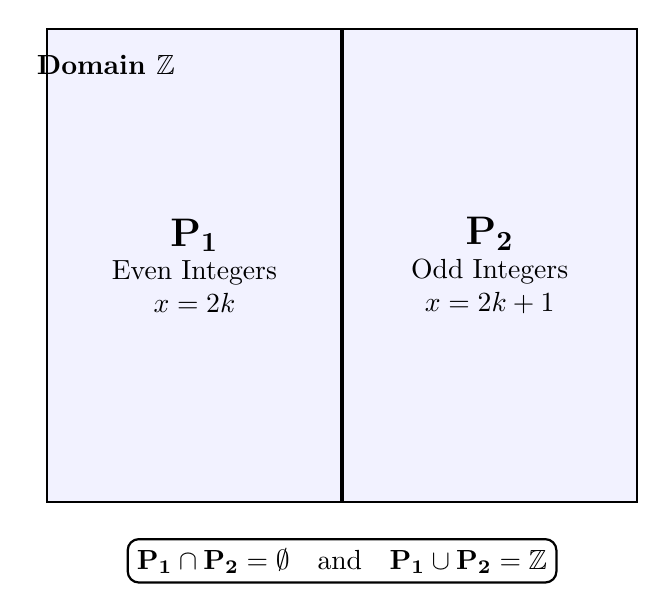
\begin{tikzpicture}[
    scale=1.5,
    set/.style={circle, draw=black, very thick, minimum size=3cm, text=black},
    partition/.style={draw=black, very thick}
]
    % Universal Set
    \draw[thick, fill=blue!5] (-2.5, -2) rectangle (2.5, 2);
    \node at (-2, 1.7) {\textbf{Domain $\Z$}};

    % Split line
    \draw[partition] (0, -2) -- (0, 2);
    
    % Labels
    \node[align=center] at (-1.25, 0) {\Large $\mathbf{P_1}$ \\ Even Integers \\ $x = 2k$};
    \node[align=center] at (1.25, 0) {\Large $\mathbf{P_2}$ \\ Odd Integers \\ $x = 2k+1$};
    
    % Condition
    \node[fill=white, draw=black, rounded corners, thick] at (0, -2.5) {$\mathbf{P_1} \cap \mathbf{P_2} = \emptyset \quad \text{and} \quad \mathbf{P_1} \cup \mathbf{P_2} = \Z$};

\end{tikzpicture}
\end{center}

\subsection{Heuristics \& "Cheats"}
\begin{itemize}
    \item \textbf{When to use Contrapositive:} If the premise involves complex algebraic mixtures (e.g., "$3x+5y$ is even") and the conclusion is simple ("$x$ and $y$ same parity"), it is almost always easier to assume the negation of the simple conclusion to build the complex premise.
    \item \textbf{When to use Contradiction:} When dealing with inequalities, rational/irrational numbers, or statements asserting non-existence.
\end{itemize}

\subsection{Pitfalls \& Fallacies}
\begin{itemize}
    \item \textbf{Affirming the Consequent (Converse Error):} Assuming $Q$ is true and deriving $P$ to prove $P \implies Q$. (Seen in Problem 3.43).
    \item \textbf{Denying the Antecedent (Inverse Error):} Assuming $\neg P$ and deriving $\neg Q$. 
    \item \textbf{False WLOG (Without Loss of Generality):} Using WLOG when the variables are \textit{not} symmetric in the underlying algebraic expression. (Seen in Problem 3.45).
\end{itemize}

\newpage

% ==========================================
% PART 5: CONCEPTUAL SYNTHESIS
% ==========================================
\section{Part 5: Conceptual Synthesis and The "Big Picture"}

\subsection{A) Thematic Connections}
The core theme of this chapter is the \textbf{formalization of exhaustive deterministic truth}. Instead of verifying truth computationally via trial (which is impossible for infinite sets like $\Z$), we map logic to set theory. Implication is subset containment; contrapositive is the complement of supersets containing complements of subsets; cases represent a disjoint union partitioning a topological or sample space. This directly unifies basic arithmetic with Boolean algebra.

\subsection{B) Forward and Backward Links}
\textbf{Backward:} This chapter rigorously grounds the intuitive arithmetic algorithms (like parity rules) taught in elementary algebra into Zermelo-Fraenkel set axioms. \\
\textbf{Forward:} The logic of partitioning domains is the direct theoretical ancestor of \textbf{$\sigma$-algebras} in Measure Theory. In probability spaces, proving an event holds almost surely (a.s.) requires partitioning the sample space $\Omega$ into disjoint measurable events (Proof by Cases) and using the Law of Total Probability, which is just the probabilistic equivalent of combining cases.

\newpage

% ==========================================
% PART 6: ABSTRACT REAL-WORLD MODELING
% ==========================================
\section{Part 6: Abstract Real-World Modeling (Quant Finance)}

\subsection{A) Concrete Scenarios}
\begin{enumerate}
    \item \textbf{Quantitative Finance (Arbitrage Pricing):} In the Cox-Ross-Rubinstein Binomial Options Pricing Model, proving that a derivative has a unique price without arbitrage relies entirely on Proof by Cases (the stock either goes UP or DOWN, partitioning the state space) and Contrapositive Logic (If Arbitrage exists $\implies$ Risk-Neutral Measure does not exist).
    \item \textbf{Machine Learning (VC Dimension Proofs):} Determining the VC dimension of a classifier often requires logical exhaustion over boolean hypercubes (parity of bits), proving by cases whether a set of points can be shattered.
\end{enumerate}

\subsection{B) Model Problem Setup: Binomial Options Model}
Let us formalize the discrete state space of a one-period financial market to demonstrate mathematical logic. Let the sample space of market states be $\Omega = \{\omega_u, \omega_d\}$ (Up state and Down state). This partitions $\Omega$.
Let $S_0$ be the stock price at $t=0$. At $t=1$, the stock price random variable is:
\[
S_1(\omega) = 
\begin{cases} 
u S_0 & \text{if } \omega = \omega_u \\
d S_0 & \text{if } \omega = \omega_d 
\end{cases}
\]
where $0 < d < 1+r < u$, and $r$ is the risk-free rate.
\textbf{Theorem:} \textit{If there is no arbitrage in the market, then there exists a unique risk-neutral probability measure $\mathbb{Q}$ such that $\E^{\mathbb{Q}}\left[\frac{S_1}{1+r}\right] = S_0$.}

\textbf{Proof Strategy Outline (Contrapositive \& Cases):}
We would prove the contrapositive: If such a measure $\mathbb{Q}$ does not exist, then an arbitrage opportunity exists.
\begin{enumerate}
    \item \textit{Assumption:} Assume no probability measure $q \in (0,1)$ exists such that $q u S_0 + (1-q) d S_0 = (1+r)S_0$.
    \item \textit{Deduction:} Solving for $q$ gives $q = \frac{(1+r)-d}{u-d}$. For $q \notin (0,1)$, Proof by Cases dictates either $1+r \le d$ or $1+r \ge u$.
    \item \textit{Case 1 ($1+r \le d$):} Borrow money at $r$, buy stock. In worst case ($\omega_d$), return is $d > 1+r$. Riskless profit (Arbitrage).
    \item \textit{Case 2 ($1+r \ge u$):} Short stock, lend money at $r$. In best case ($\omega_u$), payoff is $1+r \ge u$. Riskless profit (Arbitrage).
    \item \textit{Conclusion:} In all cases, Arbitrage exists. The contrapositive proves the Fundamental Theorem of Asset Pricing.
\end{enumerate}

\newpage

% ==========================================
% PART 7: COMMON VARIATIONS
% ==========================================
\section{Part 7: Common Variations and Untested Concepts}

The provided homework focuses strictly on the integers $\Z$ and parity (mod 2). In an advanced university setting, proof techniques must extend to \textbf{Rational vs. Irrational Numbers} (dense continuous domains) and \textbf{Modular Arithmetic beyond Mod 2}.

\textbf{Missing Concept: Proof by Contradiction with Dense Sets} \\
\textit{Theorem:} The sum of a rational number and an irrational number is irrational.
\begin{proof}
Let $a \in \Q$ and $b \notin \Q$. We prove by contradiction. Assume the conclusion is false; that is, assume $a+b \in \Q$.
Since $a \in \Q$, $a = \frac{p}{q}$ for integers $p,q$ with $q \neq 0$.
Since $a+b \in \Q$, $a+b = \frac{m}{n}$ for integers $m,n$ with $n \neq 0$.
Then $b = (a+b) - a = \frac{m}{n} - \frac{p}{q} = \frac{mq - np}{nq}$.
Since the integers are closed under multiplication and subtraction, $mq - np \in \Z$ and $nq \in \Z$ ($nq \neq 0$).
Thus, $b$ can be expressed as a ratio of integers, meaning $b \in \Q$.
This contradicts the hypothesis that $b \notin \Q$. Therefore, $a+b$ must be irrational.
\end{proof}

\newpage

% ==========================================
% PART 8: ADVANCED DIAGNOSTIC TESTING
% ==========================================
\section{Part 8: Advanced Diagnostic Testing: "Find the Flaw"}

Below are five new proofs. At first glance, they appear perfectly rigorous, but each contains a subtle, critical logical flaw. Your task is to act as the grader.

\subsection{Test Problems}

\textbf{Problem 1 (Direct Proof):}
\textit{Theorem: Let $a, b \in \Z$. If $a$ and $b$ are even, then $a+b$ is a multiple of 4.}
\begin{proof}
Assume $a$ and $b$ are even integers. By definition of even, $a = 2k$ and $b = 2k$ for some integer $k$.
We calculate the sum: $a + b = 2k + 2k = 4k$.
Since $k \in \Z$, $4k$ is a multiple of 4. Therefore, $a+b$ is a multiple of 4.
\end{proof}

\textbf{Problem 2 (Proof by Contrapositive):}
\textit{Theorem: Let $x \in \R$. If $x^2 > 0$, then $x > 0$.}
\begin{proof}
We proceed by proving the contrapositive: If $x \le 0$, then $x^2 \le 0$.
Assume $x \le 0$. 
Multiplying both sides of the inequality by $x$ gives $x \cdot x \ge 0 \cdot x$, which simplifies to $x^2 \ge 0$.
Wait, because $x$ is negative, the inequality sign flips, giving $x^2 \le 0$.
Since we proved the contrapositive, the original statement is true.
\end{proof}

\textbf{Problem 3 (Proof by Cases):}
\textit{Theorem: For all $x \in \R$, $\frac{x^2 - 1}{x - 1} = x + 1$.}
\begin{proof}
We proceed by exhaustive cases on the sign of $x$.
Case 1 ($x > 0$): We factor the numerator: $\frac{(x-1)(x+1)}{x-1}$. Canceling $x-1$ yields $x+1$.
Case 2 ($x \le 0$): We factor the numerator identically: $\frac{(x-1)(x+1)}{x-1}$. Canceling $x-1$ yields $x+1$.
Since it holds for all cases, the theorem is proven for all real numbers.
\end{proof}

\textbf{Problem 4 (Biconditional Proof):}
\textit{Theorem: Let $A, B$ be sets. $A \subseteq B \iff A \cup B = B$.}
\begin{proof}
Assume $A \subseteq B$. Let $x \in A \cup B$. Then $x \in A$ or $x \in B$. Since $A \subseteq B$, if $x \in A$, then $x \in B$. Thus, in either case, $x \in B$. This shows $A \cup B \subseteq B$. Since $B \subseteq A \cup B$ is trivially true, $A \cup B = B$.
Because we have established the equality using logical steps, the equivalence $A \subseteq B \iff A \cup B = B$ holds by definition of set theory.
\end{proof}

\textbf{Problem 5 (WLOG Trick):}
\textit{Theorem: Let $x,y \in \Z$. If $xy$ is even, then both $x$ and $y$ are even.}
\begin{proof}
Assume $xy$ is even. By prime factorization, 2 must divide the product $xy$. 
Without loss of generality (WLOG), assume 2 divides $x$. 
Therefore, $x = 2k$ for some integer $k$. Thus, $x$ is even. 
Since the variables $x$ and $y$ are symmetric, we can swap their labels, proving $y$ is also even. 
Hence, both $x$ and $y$ are even.
\end{proof}

\vspace{2cm}

\subsection{Solution Key: Flaws Revealed}

\textbf{Flaw 1 (Variable Dependency Error):} By setting $a=2k$ and $b=2k$, the author assumed $a=b$. Two independent variables must be assigned independent arbitrary constants ($a=2k$, $b=2m$). The sum is $2(k+m)$, which is even, but not necessarily a multiple of 4 (e.g., $a=2, b=4$, sum is 6).

\textbf{Flaw 2 (Algebraic Manipulation Error):} The contrapositive statement is correctly identified, but the algebra is flawed. If $x=0$, multiplying by $x$ doesn't flip the sign. If $x < 0$, $x^2 \ge 0$. The statement $x^2 \le 0$ is actually false for $x < 0$. The theorem itself is false (counterexample $x=-2$, $x^2=4>0$, but $-2 \ngtr 0$).

\textbf{Flaw 3 (Division by Zero ignored in partition):} The partition is $\{x > 0\}$ and $\{x \le 0\}$, which covers $\R$. However, the expression is undefined at $x=1$, which falls into Case 1. The cancellation step divides by zero when $x=1$.

\textbf{Flaw 4 (Missing Converse):} The proof only establishes the forward direction ($\implies$). Proving a biconditional requires assuming $A \cup B = B$ and deriving $A \subseteq B$ in a separate logical block. 

\textbf{Flaw 5 (Symmetry Abuse & Converse Error):} The theorem itself is false (if $x=2, y=3$, $xy=6$ is even, but $y$ is odd). WLOG cannot be used to force $y$ to have the same property as $x$. WLOG just means "it doesn't matter whether 2 divides $x$ or $y$." It proves \textit{at least one} is even, not \textit{both}.

\end{document}